\section{CNN Based Road User Detection Using the 3D Radar
Cube}\label{header-n359}

\emph{IEEE ROBOTICS AND AUTOMATION LETTERS, VOL. 5, NO. 2, APRIL 2020}
{[}8{]}

\subsection{Introduction}\label{header-n361}

Radars are attractive sensors for intelligent vehicles as they are
relatively robust to weather and lighting conditions (e.g. rain, snow,
darkness) compared to camera and LIDAR sensors. They also have excellent
range sensitivity and can measure radial object velocities directly
using the Doppler effect. A radar outputs a point-cloud of reflections
called \emph{radar targets} in every frame and each radar target has the
following features: range $r$ and azimuth $\alpha$, radar cross
section RCS (i.e. reflectivity), and the object's radial speed $v_r$
relative to the ego-vehicle. The authors call these feature
\emph{target-level}. Many radar-based road user detection methods first
cluster radar targets by their \emph{target-level} features. Object
detection and classification methods depend on the success of this
initial classification step. Other methods explore using the
\emph{low-level radar cube} given by early processing of the radar
signal. The radar cube is a 3D data matrix with axes corresponding to
range, azimuth, and velocity (also called Doppler). In contrast to the
target-level data, the radar cube provides the complete speed
distribution (i.e. Doppler vector) at multiple 2D range-azimuth
locations. Such distributions can capture modulations of an object's
main velocity caused by its moving parts, e.g. swinging limbs or
rotating wheels. In this work, the authors show that these data can be
used as valuable features for object classification. The features
derived from a 3D cube are called \emph{low-level}. This work focus only
on addressing moving road users. In \emph{Prophet}, proposed in
{[}10{]}, radar targets are first clustered into objects by DBSCAN.
Then, several cluster-wise features are extracted, e.g. the
variance/mean of $v_r$ and $r$. The performance of various
classifiers (Random Forest, Support Vector Machine (SVM), 1-layer Neural
Network, etc.) were compared in a single-class (pedestrian) detection
task. The Schumann method {[}11{]} also uses clusters calculated by
DBSCAN as the base of a multi-class (car, pedestrian, group of
pedestrians, cyclist, truck) detection, but extract different features,
e.g. deviation and spread of α (azimuth). In this letter, the authors
propose a radar-based, multi-class moving road user detection method,
which exploits both expert knowledge at the \emph{target-level}
(accurate 2D location, addressed phase ambiguity), and \emph{low-level}
information from the full 3D radar cube rather than a 2D projection. The
method's core is a Convolutional Neural Network (CNN) called Radar
Target Classification Network (\emph{RTCnet}). The inclusion of
low-level data enables the classification of individual radar targets
before any object clustering; the latter step can benefit from the
obtained class scores.

\subsection{Proposed method}\label{header-n363}

\emph{RTCnet} classifies each target individually based on the fused
low-level and target-level data. The network consists of three parts.
The first encodes the data in spatial domains (range, azimuth) and
grasps the surroundings' Doppler distribution. The second is applied to
this output to extract class information from the distribution of speed.
Finally, the third part provides classifications scores by two fully
connected layers (FC). The output is either multi-class (one score for
each class) or binary. In the latter case, an ensemble voting step
combines the result of several binary classifiers. A class-specific
clustering step (i.e. the radar targets' predicted class information is
used) generates an object list output. The following figure shows an
overview of our method.

\begin{figure}[h!]
\centering
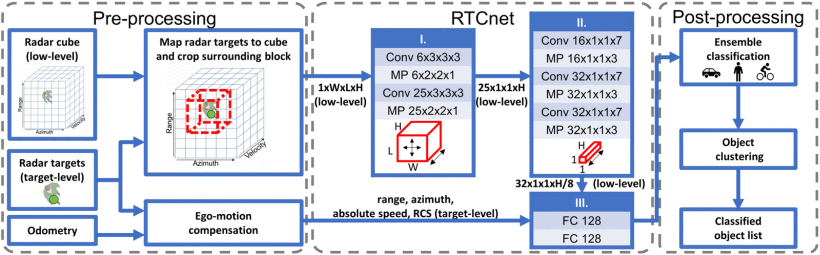
\includegraphics[width=0.95\linewidth]{images/pipelineoverview.png}
\caption{The proposed pipeline's architecture}
\end{figure}

\subsubsection{Pre-Processing}\label{header-n366}

Every single frame of radar targets and a single frame of the radar cube
(low-level data) is fetched and pre-processed. First, radar targets with
low compensated (absolute) velocity are considered as static and are
filtered out. Then, corresponding target-level and low-level radar data
are connected. Next, we look up each remaining dynamic radar target,
such as a grid cell in the radar cube based on their reported range,
azimuth, and (relative) velocity ($r$, $\alpha$, $v_r$).
Afterward, a 3D block of the radar cube is cropped around each radar
target's grid cell with radius in range/azimuth/Doppler dimensions
($L$, $W$, $H$).

\subsubsection{Network}\label{header-n368}

The \emph{RTCnet} structure can be seen in detail in the figure above.
The network is composed of three modules:

\begin{itemize}
\item
  \textbf{Down-Sample Range and Azimuth Dimensions:} it aims to encode
  the radar target's spatial neighborhood's Doppler distribution into a
  tensor without extension in range or azimuth. In other words, it
  transforms the $1 \times W \times L \times H$ sized data to a $C \times 1 \times 1
  \times H$ sized tensor (sizes are given as $Channel \times Azimuth \times Range \times
  Doppler$), where $C$ was chosen as 25. To do this, it contains two 3D
  convolutional layers (Conv) followed by two maxpool layers (MP).
\item
  \textbf{Process Doppler Dimension:} the aim of this module is to
  extract class information from the speed distribution around the
  target. It operates on the output of the first which is $25 \times 1 \times 1 \times
  H$. To do this, two 1D convolutions along the Doppler dimension are
  applied, each of them is followed by a maxpool layer. The output of
  this module is a $32 \times 1 \times 1 \times H/8$ block.
\item
  \textbf{Score Calculation:} The output of the second module is
  flattened and concatenated to the \emph{target-level} features ($r$,
  $\alpha$, $v_r$, $RCS$) and used by this module. It uses two
  fully connected layers with 128 nodes each to provide scores. The
  output layer has either four nodes (one for each class) for
  multi-class classification or two for binary tasks.
\end{itemize}

\subsubsection{Ensemble Classifying}\label{header-n377}

It is possible to train the third module to perform multi-class
classification directly. It implements also an ensemble voting system of
binary classifiers, in the case of the network has two output nodes.
This module is trained as One-vs-All (OvA) and One-vs-One (OvO) binary
classifiers for each class (e.g. car-vs-all) and pair of classes (e.g.
car-vs-cyclist), 10 in total.

\subsubsection{Object Clustering}\label{header-n379}

To obtain proposals for object detection, the authors cluster the
classified radar targets with DBSCAN incorporating the predicted class
information. The radar targets with bike/pedestrian/car predicted labels
are clustered in separate steps. As a metric, we used a spatial
threshold $\gamma_{xy}$ on the Euclidean distance in the $x, y$
space, and a separate speed threshold $\gamma_v$ in velocity
dimension. The advantage of clustering each class separately is that no
universal parameter set is needed for DBSCAN. The authors use different
parameters for different classes, e.g. larger radius for cars and small
ones for pedestrians. Furthermore, swapping the clustering and
classification step makes it possible to consider objects with a single
reflection. The following figure reports three challenging cases for the
cluster classification:

\begin{itemize}
\item
  \textbf{A:} objects may be clustered together (red circle)
\item
  \textbf{B:} large objects may be split up into several clusters
\item
  \textbf{C:} object with only one reflection
\end{itemize}

\begin{figure}[h!]
\centering
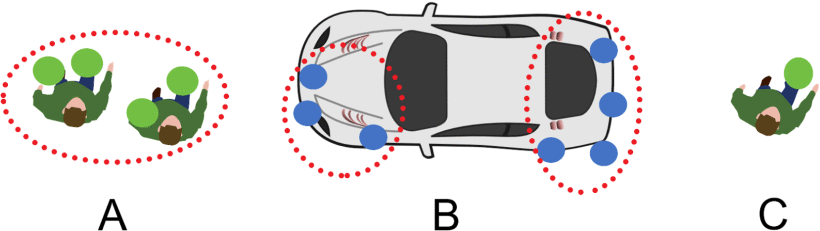
\includegraphics[width=0.95\linewidth]{images/clusteringdiff.png}
\caption{Challenging cases for cluster-wise classification methods}
\end{figure}

To address this, the method performs a filtering on the produced object
proposals, calculating their spatial, velocity, and class score
distribution distances. If two clusters have different classes and are
close enough in all dimensions, they are merged the smaller class to the
larger (i.e. pedestrians to cyclists and cars, cyclists to cars).

\subsubsection{Dataset}\label{header-n390}

The dataset is obtained in the real-world with a demonstration vehicle
during a time of an hour. There are recorded both the target-level and
low-level output of our radar, the output of a stereo camera ($1936 \times
1216$ px), and the vehicle's odometry (filtered location and ego-speed).
Annotation was fetched automatically from the camera sensor using the
Single Shot Multibox Detector (SSD) {[}9{]}. Then, the mislabeled ground
truth are corrected manually. To further extend the training dataset,
the authors augmented the data by mirroring the radar frames and adding
a zero-mean, 0.05 std Gaussian noise to the normalized \emph{r} and
\emph{v\textsubscript{r}} features. Training and testing sets are from
two independent driving (33 and 31 minutes long) which took place on
different days and routes. The validation set is a 10\% split of
training dataset after shuffling.

\subsection{Experiments}\label{header-n392}

The proposed method is tested in two different experiments:

\begin{itemize}
\item
  \textbf{Experiment 1:} the classification task's performances are
  examined. As target-wise metric, a true positive is a correctly
  classified target. For cluster-wise methods, the predicted label of a
  cluster is assigned to each radar target inside it. Furthermore, the
  authors also performed an ablation study to see how different features
  benefit the method. \emph{RTCnet (no ensemble)} is a single,
  multi-class network to see if ensembling is beneficial. \emph{RTCnet
  (no RCS)} is identical to RTCnet, but the RCS target-level feature is
  removed to examine its importance. Similarly, in \emph{RTCnet (no
  speed)} the absolute speed of the targets is unknown to the networks,
  only the relative speed distribution (in the low-level data) is given.
  Finally, \emph{RTCnet (no low-level)} is a significantly modified
  version as it only uses target-level features.
\item
  \textbf{Experiment 2:} this experiment consists of comparing the
  methods in object detection task, examining the entire pipeline.
  Predictions and annotations are compared by their intersection and
  union calculated in number of targets. A true positive is a prediction
  which has an Intersection Over Union (IoU) bigger than or equal to 0.5
  with an annotated object. Further detections of the same ground truth
  object count as false positives. To better understand this metric, see
  the figure below.
\newpage
  \begin{figure}[h!]
  \centering
  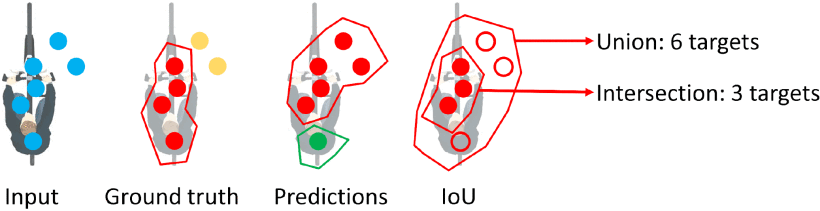
\includegraphics[width=0.95\linewidth]{images/iuo.png}
  \caption{Object-level metric. $Intersection / Union \geq 0.5$ counts as a true positive. In this example, there is a true positive cyclist and a false positive pedestrian detection.}
  \end{figure}
\end{itemize}

We selected Schumann {[}11{]} as a baseline because it is the only
multi-object, multi-class detection method found with small latency.
Also, \emph{Prophet} {[}1{]} is selected as a baseline. Since the DBSCAN
parameters are sensor-specific, the following table shows the optimal
parameters for the two baselines and for the class-specific clusters.
Both baselines method has the parameter \emph{v\textsubscript{min}},
used to find the static radar targets.

\begin{longtable}[]{@{}lllll@{}}
\toprule
\textbf{Method} & \textbf{$\mathbold{\gamma_{xy}}$} & \textbf{$\mathbold{  \gamma_v}$} &
\textbf{\emph{Min Points}} & \textbf{$\mathbold{ v_{  min}}$}\tabularnewline
\midrule
\endhead
\emph{Prophet} & 1.2 $m$ & 1.3 $m / s$ & 2 & 0.4
$m / s$\tabularnewline
\emph{Schumann} & 1.3 $m$ & 1.4 $m / s$ & 2 & 0.4
$m / s$\tabularnewline
Class specific: peds. & 0.5 $m$ & 2.0 $m / s$ & 1 & -\tabularnewline
Class specific: cyclists & 1.6 $m$ & 1.5 $m / s$ & 2 &
-\tabularnewline
Class specific: cars & 4.0 $m$ & 1.0 $m / s$ & 3 & -\tabularnewline
\bottomrule
\caption{Optimized DBSCAN parameters for the two baselines and the proposed method}
\end{longtable}

For two baselines, the classifiers consists of a Random Forest with 50
trees. The size of the cropped block are set to $L = W = 5, H = 32$.
The speed threshold to filter out static objects is a sensor-specific
parameter and was set to 0.3 \emph{m / s} based on empirical evidence.
The thresholds to merge clusters during object clustering were set to 1
$m$ spatially, 0.6 for scores, 2 $m / s$for pedestrian to cyclist,
and 1.2 $m / s$ for pedestrian/cyclist to car merges. The input data
are normalized to be zero-mean and have a standard deviation of 1.

\newpage
\subsection{Results}\label{header-n439}

\subsubsection{Experiments results}\label{header-n440}

The results of \emph{experiment 1} (target classification) are presented
in the following table.

\begin{longtable}[]{@{}llllll@{}}
\toprule
\textbf{Method} & \textbf{Pedestrian} & \textbf{Cyclist} & \textbf{Car}
& \textbf{Other} & \textbf{Avg}\tabularnewline
\midrule
\endhead
\emph{Prophet} & 0.61 & 0.58 & 0.34 & 0.91 & 0.61\tabularnewline
\emph{Schumann} & 0.67 & \textbf{0.68} & 0.46 & \textbf{0.92} &
0.68\tabularnewline
\emph{RTCnet (no low-level)} & 0.56 & 0.63 & 0.33 & 0.90 &
0.61\tabularnewline
\emph{RTCnet (no speed)} & 0.66 & 0.63 & 0.36 & 0.91 &
0.64\tabularnewline
\emph{RTCnet (no RCS)} & \textbf{0.71} & 0.66 & 0.48 & 0.91 &
0.69\tabularnewline
\emph{RTCnet (no ensemble)} & 0.67 & 0.65 & 0.47 & 0.89 &
0.67\tabularnewline
\emph{RTCnet} & \textbf{0.71} & 0.67 & \textbf{0.50} & \textbf{0.92} &
\textbf{0.70}\tabularnewline
\bottomrule
\caption{Target-wise scores divided per class obtained by the tested approaches}
\end{longtable}

\emph{RTCnet} outperformed the two cluster-wise baselines reaching an
average score of 0.70. \emph{Schumann} has slightly better results on
cyclists than \emph{RTCnet} (0.68 vs 0.67) but performs significantly
worse on pedestrians (0.67 vs 0.71) and cars (0.46. vs 0.50). The
ablation study showed that removing each feature yields worse results
than the complete pipeline, with the exception of \emph{RTCnet (no RCS)}
which has an average of 0.69. The results also show that classification
performance changes over the distance from the target object and the
vehicle, based on the number of samples in the training set. The figure
below shows this fact.

\begin{figure}[h!]
\centering
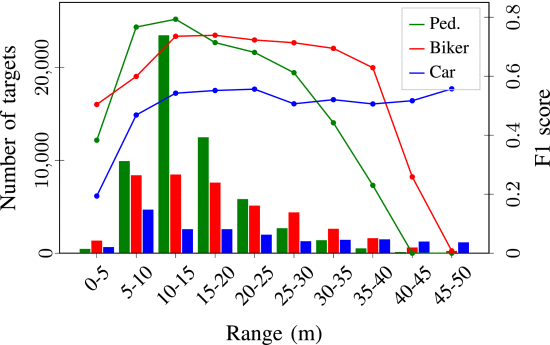
\includegraphics[width=0.85\linewidth]{images/resultsdistance.png}
\caption{Target-wise scores (lines) and number of targets in training set (bars) in function of distance from vehicle}
\end{figure}

For \emph{experiment 2} (object detection), the results are shown in the
following table.

\begin{longtable}[]{@{}lllll@{}}
\toprule
\textbf{Method} & \textbf{Pedestrian} & \textbf{Cyclist} & \textbf{Cars}
& \textbf{Avg.}\tabularnewline
\midrule
\endhead
\emph{Prophet} & 0.48 & 0.50 & 0.23 & 0.40\tabularnewline
\emph{Schumann} & 0.54 & \textbf{0.60} & 0.31 & 0.48\tabularnewline
\emph{RTCnet} & \textbf{0.61} & 0.59 & \textbf{0.47} &
\textbf{0.56}\tabularnewline
\bottomrule
\caption{Object-wise results obtained by the baselines and the proposed method}
\end{longtable}

\emph{RTCnet} reached slightly worse results on cyclists than
\emph{Schumann} (0.59 vs 0.60), but significantly outperformed it on
pedestrians (0.61 vs 0.54), cars (0.47 vs 0.31), and in average (0.56 vs
0.48).

\subsubsection{Discussion}\label{header-n528}

The proposed method outperformed the baselines in target classification
mainly due to two reasons. First, the classification does not depend on
a clustering step. This allows us to handle objects that contain a
single radar target (a common occurrence, especially for pedestrians)
and mitigates the difficult cases shows in the figure above. Second, the
method uses the low-level radar data, which brings the information of
the speed distribution around the radar target. To demonstrate that this
inclusion is beneficial, the authors show that only using target-level
data and only the third module of the network (\emph{RTCnet (no
low-level)}) caused a significant drop in performance from 0.70 to 0.61
average score. The results of RTCnet (no low-level) and RTCnet (no
speed) prove that the relative velocity distribution (i.e. the low-level
radar data) indeed contains valuable class information. Despite the
radar's performances are uniform in darkness/shadows/bright
environments, its typical errors are shown in the following figure.
Radar is easily reflected by flat surfaces (e.g. side of cars) acting
like mirrors, creating ghost targets.

\begin{figure}[h!]
\centering
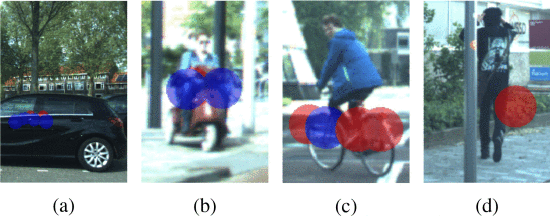
\includegraphics[width=0.85\linewidth]{images/rtcnetfails.png}
\caption{Examples of radar targets misclassified by RTCnet}
\end{figure}

The combination of the proposed network and the clustering step
outperformed the baseline methods in the object detection task. This is
mainly because by swapping the clustering and classifying steps, classes
can be clustered with different parameters. This is mainly because by
swapping the clustering and classifying steps, classes can be clustered
with different and more appropriate parameters.

\subsection{Conclusions}\label{header-n532}

In extensive experiments on a real-life dataset, the authors showed that
the proposed method improves upon the baselines in target-wise
classification by reaching an average score of 0.70 (vs. 0.68
\emph{Schumann}). Furthermore, the importance of low-level features and
ensembling in an ablation study is demonstrated. Furthermore, the
authors show that the proposed method outperforms the baselines overall
in object-wise classification by yielding an average score of 0.56 (vs.
0.48 \emph{Schumann}).